\documentclass{article}\usepackage[]{graphicx}\usepackage[]{color}
%% maxwidth is the original width if it is less than linewidth
%% otherwise use linewidth (to make sure the graphics do not exceed the margin)
\makeatletter
\def\maxwidth{ %
  \ifdim\Gin@nat@width>\linewidth
    \linewidth
  \else
    \Gin@nat@width
  \fi
}
\makeatother

\definecolor{fgcolor}{rgb}{0.345, 0.345, 0.345}
\newcommand{\hlnum}[1]{\textcolor[rgb]{0.686,0.059,0.569}{#1}}%
\newcommand{\hlstr}[1]{\textcolor[rgb]{0.192,0.494,0.8}{#1}}%
\newcommand{\hlcom}[1]{\textcolor[rgb]{0.678,0.584,0.686}{\textit{#1}}}%
\newcommand{\hlopt}[1]{\textcolor[rgb]{0,0,0}{#1}}%
\newcommand{\hlstd}[1]{\textcolor[rgb]{0.345,0.345,0.345}{#1}}%
\newcommand{\hlkwa}[1]{\textcolor[rgb]{0.161,0.373,0.58}{\textbf{#1}}}%
\newcommand{\hlkwb}[1]{\textcolor[rgb]{0.69,0.353,0.396}{#1}}%
\newcommand{\hlkwc}[1]{\textcolor[rgb]{0.333,0.667,0.333}{#1}}%
\newcommand{\hlkwd}[1]{\textcolor[rgb]{0.737,0.353,0.396}{\textbf{#1}}}%
\let\hlipl\hlkwb

\usepackage{framed}
\makeatletter
\newenvironment{kframe}{%
 \def\at@end@of@kframe{}%
 \ifinner\ifhmode%
  \def\at@end@of@kframe{\end{minipage}}%
  \begin{minipage}{\columnwidth}%
 \fi\fi%
 \def\FrameCommand##1{\hskip\@totalleftmargin \hskip-\fboxsep
 \colorbox{shadecolor}{##1}\hskip-\fboxsep
     % There is no \\@totalrightmargin, so:
     \hskip-\linewidth \hskip-\@totalleftmargin \hskip\columnwidth}%
 \MakeFramed {\advance\hsize-\width
   \@totalleftmargin\z@ \linewidth\hsize
   \@setminipage}}%
 {\par\unskip\endMakeFramed%
 \at@end@of@kframe}
\makeatother

\definecolor{shadecolor}{rgb}{.97, .97, .97}
\definecolor{messagecolor}{rgb}{0, 0, 0}
\definecolor{warningcolor}{rgb}{1, 0, 1}
\definecolor{errorcolor}{rgb}{1, 0, 0}
\newenvironment{knitrout}{}{} % an empty environment to be redefined in TeX

\usepackage{alltt}
\usepackage{natbib}
\usepackage[unicode=true]{hyperref}
\usepackage{geometry}
\usepackage{amsmath}
\geometry{tmargin=1in,bmargin=1in,lmargin=1in,rmargin=1in}


\IfFileExists{upquote.sty}{\usepackage{upquote}}{}
\begin{document} 
\title{STAT243-PS7}
\author{Jinhui Xu}
\date{Nov. 2017}

\maketitle


I work with Xin Shi, Xiao Li, Shan Gao, Zicheng Huang, Junyuan Gao, Junyi Tang

\section{Question 1}

From 1000 estimates of coefficent, we can calculate an standard error $\hat{se^*}$ of these 1000 estimates.\\
From 1000 standard errors :assume that $se_1\leq se_2...\leq se_{1000}$, we can get a 95\% confidence interval $[se_{26},se_{975}]$ \\
The standard error properly characterizes the uncertainty of the estimated regression coefficient if $\hat{se^*}$ falls into the above 95\% confidence interval.

\section{Question 2}
\begin{align*}
  ||A||_2&=\sup_{||z||_2=1}\sqrt{(Az)^T(Az)}\\
  \end{align*}
As A is symmetric, it can be written as $A=U\Sigma U^T$, where U is a basis of $R^n$, $UU^T=U^TU=I$ and $\Sigma=\begin{bmatrix}\lambda_1&&\\&\ddots&\\&&\lambda_n\end{bmatrix}$. Then any vector $z\in R^n$ can be written as $U\times z^*$, where $z^*=(z_1,z_2,...,z_n)$ is the coordinates of z in the basis of U.\\
In this way, we can compute Az as follows:\\
\begin{align*}
  Az&=U\Sigma U^T \times z\\
    &=U\Sigma U^T \times U\times z^*\\
    &=U\Sigma \times z^*
  \end{align*}
  
  
Then we can compute $\sqrt{(Az)^T(Az)}$ :\\
\begin{align*}
  \sqrt{(Az)^T(Az)}&=\sqrt{(U\Sigma \times z^*)^T(U\Sigma \times z^*)}\\
                   &=\sqrt{(z^*)^T\Sigma U^T\times U\Sigma z^*}\\
                   &=\sqrt{(z^*)^T(\Sigma)^2z^*}\\
                   &=\sqrt{\sum_{i=1}^{n}\lambda_i^2z_i^2}
  \end{align*}


In this way, when $||z||_2=1$
\begin{align*}
  \sqrt{(Az)^T(Az)}&\leq \sqrt{max(\lambda_i^2)}\\
                   &=max|\lambda_i|
  \end{align*}
  
  
  Assume $|\lambda_j|=max|\lambda_i|, i=1,...,n$, then let $z^*=\begin{bmatrix}0&\cdots0&1&0&\cdots&0\end{bmatrix}^T\longrightarrow$ 1 at $j$th element, which can satifies the equation:
  \begin{align*}
  \sqrt{(Az)^T(Az)}&=\sqrt{\sum_{i=1}^{n}\lambda_i^2z_i^2}\\
                   &=|\lambda_j|\\
                   &=max|\lambda_i|
  \end{align*}
  
which means that $||A||_2=\sup_{||z||_2=1}\sqrt{(Az)^T(Az)}=max|\lambda_i|$ \\

\section{Question 3}
\subsection{(a)}
According to SVD, A always can be decomposed as 
$$A=UDV^T,\qquad D=\begin{bmatrix}\lambda_1&&\\&\ddots&\\&&\lambda_n\end{bmatrix}$$
where U, V are matrics with althonormal columns which means that $U^TU=I, V^TV=I$, then 
\begin{align*}
  X=UDV^T&\Longrightarrow X^TX=VDU^TUDV^T=VD^2V^T\\
         &\Longrightarrow X^TX\times V=VD^2V^TV=VD^2=\begin{bmatrix}\lambda_1^2v_1,&\cdots&,\lambda_n^2v_n\end{bmatrix}\qquad
         \text{$v_i$ is column vector of V}
  \end{align*}
Therefore, V are eigenvectors of $X^TX$ and the corresponding eigenvalues are the diagonal values of $D^2$, which equals to the squares of diagonal values of D{(the squares of the singular values of X)}.\\

Proof of semi-positive for $X^TX$ 
$$\forall y \in R^n \qquad y^TX^TXY=(Xy)^T(Xy)=||Xy||^2\geq 0$$

\subsection{(b)}

If we have computed the eigendecomposition of $\Sigma$, $\Sigma=UDU^T$ where $U^TU=I, D=\begin{bmatrix}\lambda_1&&\\&\ddots&\\&&\lambda_n\end{bmatrix}$\\
Then we can write cI as $cI=UCU^T$, where $C=\begin{bmatrix}c&&\\&\ddots&\\&&c\end{bmatrix}$\\
In this way, 
$$Z=\Sigma + cI=UDU^T+UCU^T=U(C+D)U^T$$
where $C+D=\begin{bmatrix}\lambda_1+c&&\\&\ddots&\\&&\lambda_n+c\end{bmatrix}$, so the eigenvalues of Z are $\lambda_1+c,...,\lambda_n+c$, which need n additions.


\section{Question 4}
\subsection{(a)}
As QR decomposition has less computation cost and be more stable than Cholesky decomposition, I first do QR decomposition for X.Then :$$C=X^TX=(QR)^T(QR)=R^TQ^TQR=R^TR$$
Calculate $\hat{\beta}$
\begin{align*}
\hat{\beta}&=(R^TR)^{-1}d+(R^TR)^{-1}A^T(A(R^TR)^{-1}A^T)^{-1}(-A(R^TR)^{-1}d+b)\\
           &=(R^TR)^{-1}d+(R^TR)^{-1}A^T((AR^{-1})(AR^{-1})^T)^{-1}(-A(R^TR)^{-1}d+b)
  \end{align*}
As $R^TR$ and $R$ are both upper triangular matrics, we can use backsolve to do above computation. R code just like the following:

\begin{knitrout}
\definecolor{shadecolor}{rgb}{0.969, 0.969, 0.969}\color{fgcolor}\begin{kframe}
\begin{alltt}
\hlstd{QR_beta}\hlkwb{<-}\hlkwd{backsolve}\hlstd{(R,} \hlkwd{backsolve}\hlstd{(R,}
              \hlkwd{t}\hlstd{(X)}\hlopt \hlstd{Y}\hlopt{+} \hlkwd{t}\hlstd{(A)} \hlopt \hlkwd{backsolve}\hlstd{(AR,}\hlkwd{backsolve}\hlstd{(AR,}\hlopt{-}\hlstd{A}\hlopt\hlkwd{backsolve}\hlstd{(R,} \hlkwd{t}\hlstd{(Q)}\hlopt\hlstd{Y)}
                  \hlopt{+}\hlstd{b,}\hlkwc{transpose}\hlstd{=T)),}\hlkwc{transpose}\hlstd{=T))}
\end{alltt}
\end{kframe}
\end{knitrout}

\subsection{(b)}
First define two function to calculate $\hat{\beta}$, one uses QR decomposition, the other one uses solve to inverse matrics.

\begin{knitrout}
\definecolor{shadecolor}{rgb}{0.969, 0.969, 0.969}\color{fgcolor}\begin{kframe}
\begin{alltt}
\hlcom{#define the function which uses QR decomposition }
\hlstd{QR_beta}\hlkwb{<-}\hlkwa{function}\hlstd{(}\hlkwc{A}\hlstd{,}\hlkwc{X}\hlstd{,}\hlkwc{Y}\hlstd{,}\hlkwc{b}\hlstd{)\{}

  \hlcom{#get Q, R of in QR decompodition of X}
  \hlstd{X_R}\hlkwb{<-}\hlkwd{qr.R}\hlstd{(}\hlkwd{qr}\hlstd{(X))}
  \hlstd{X_Q}\hlkwb{<-}\hlkwd{qr.Q}\hlstd{(}\hlkwd{qr}\hlstd{(X))}

  \hlcom{#get R in QR decomposition of AR^\{-1\}}
  \hlstd{AR_R}\hlkwb{<-}\hlkwd{qr.R}\hlstd{(}\hlkwd{qr}\hlstd{(}\hlkwd{t}\hlstd{(A}\hlopt\hlkwd{solve}\hlstd{(X_R))))}

  \hlcom{#calculate beta hat in the same way in question (a)}
  \hlstd{beta}\hlkwb{<-}\hlkwd{backsolve}\hlstd{(X_R,} \hlkwd{backsolve}\hlstd{(X_R,} \hlkwd{t}\hlstd{(X)}\hlopt\hlstd{Y}\hlopt{+}\hlkwd{t}\hlstd{(A)}\hlopt
                                   \hlkwd{backsolve}\hlstd{(AR_R,}\hlkwd{backsolve}\hlstd{(AR_R,}
                                             \hlopt{-}\hlstd{A}\hlopt\hlkwd{backsolve}\hlstd{(X_R,} \hlkwd{t}\hlstd{(X_Q)}\hlopt\hlstd{Y)}\hlopt{+}\hlstd{b,}\hlkwc{transpose}\hlstd{=T)),}
                                 \hlkwc{transpose}\hlstd{=T))}
 \hlkwd{return}\hlstd{(beta)}
\hlstd{\}}

\hlcom{#define the function of methods which uses solve to calculate the inverse of matrics}
\hlstd{solve_beta}\hlkwb{<-}\hlkwa{function}\hlstd{(}\hlkwc{A}\hlstd{,}\hlkwc{X}\hlstd{,}\hlkwc{Y}\hlstd{,}\hlkwc{b}\hlstd{)\{}
    \hlstd{d}\hlkwb{<-}\hlkwd{t}\hlstd{(X)}\hlopt\hlstd{Y}
    \hlkwd{solve}\hlstd{(}\hlkwd{crossprod}\hlstd{(X))}\hlopt\hlstd{d}\hlopt{+}
             \hlkwd{solve}\hlstd{(}\hlkwd{crossprod}\hlstd{(X))}\hlopt\hlkwd{t}\hlstd{(A)}\hlopt
                  \hlkwd{solve}\hlstd{(A}\hlopt\hlkwd{solve}\hlstd{(}\hlkwd{crossprod}\hlstd{(X))}\hlopt\hlkwd{t}\hlstd{(A))}\hlopt\hlstd{(}\hlopt{-}\hlstd{A}\hlopt\hlstd{(}\hlkwd{solve}\hlstd{(}\hlkwd{crossprod}\hlstd{(X))}\hlopt\hlstd{d)}\hlopt{+}\hlstd{b)}
\hlstd{\}}
\end{alltt}
\end{kframe}
\end{knitrout}

Then I give an example to examine the efficency of QR decomposition
\begin{knitrout}
\definecolor{shadecolor}{rgb}{0.969, 0.969, 0.969}\color{fgcolor}\begin{kframe}
\begin{alltt}
\hlcom{#set basic parameters}
\hlstd{m}\hlkwb{<-}\hlnum{100}
\hlstd{n}\hlkwb{<-}\hlnum{1000}
\hlstd{p}\hlkwb{<-}\hlnum{1000}
\hlstd{A}\hlkwb{<-}\hlkwd{matrix}\hlstd{(}\hlkwd{rnorm}\hlstd{(m}\hlopt{*}\hlstd{p),m)}
\hlstd{X}\hlkwb{<-}\hlkwd{matrix}\hlstd{(}\hlkwd{rnorm}\hlstd{(n}\hlopt{*}\hlstd{p),n)}
\hlstd{Y}\hlkwb{<-}\hlkwd{rnorm}\hlstd{(n)}
\hlstd{b}\hlkwb{<-}\hlkwd{rnorm}\hlstd{(m)}
\hlstd{d}\hlkwb{<-}\hlkwd{t}\hlstd{(X)}\hlopt\hlstd{Y}

\hlcom{#compare the result of two methods}
\hlkwd{solve_beta}\hlstd{(A,X,Y,b)[}\hlnum{1}\hlopt{:}\hlnum{5}\hlstd{]}
\end{alltt}
\begin{verbatim}
## [1] -0.276921371  0.005403068 -0.067521364  0.035844192 -0.158073372
\end{verbatim}
\begin{alltt}
\hlkwd{QR_beta}\hlstd{(A,X,Y,b)[}\hlnum{1}\hlopt{:}\hlnum{5}\hlstd{]}
\end{alltt}
\begin{verbatim}
## [1] -0.276921371  0.005403068 -0.067521364  0.035844192 -0.158073372
\end{verbatim}
\begin{alltt}
\hlcom{#compare the time used to run the two functions}
\hlkwd{system.time}\hlstd{(}\hlkwd{solve_beta}\hlstd{(A,X,Y,b))}
\end{alltt}
\begin{verbatim}
##    user  system elapsed 
##   6.322   0.083   6.597
\end{verbatim}
\begin{alltt}
\hlkwd{system.time}\hlstd{(}\hlkwd{QR_beta}\hlstd{(A,X,Y,b))}
\end{alltt}
\begin{verbatim}
##    user  system elapsed 
##   2.426   0.054   2.590
\end{verbatim}
\end{kframe}
\end{knitrout}

From the result, we can see QR decomposition runs faster and gets the same result with the oridinary method. In addition, as we know, the advantage in speed can be much more obvious when p is larger. Therefore, using QR decomposition should be a better choice when we face large dimension matrics multiplication.


\section{Question 5}
\subsection{(a)}
Although X, Z are sparse, $\hat{X}$ can be dense matrics. So it may take large memory use. And in this way, calculating $\hat{\beta}$ also has large computation cost and takes large memory use.
So we can not do calculation in that way.

\subsection{(b)}
As X, Z are both sparse, we can combine two equations and only use X and Z to calculate the value of $\hat{\beta}$

\begin{align*}
\hat{X}=Z(Z^TZ)^{-1}Z^TX&\Longrightarrow \hat{X}^T\hat{X}=(Z(Z^TZ)^{-1}Z^TX)^TZ(Z^TZ)^{-1}Z^TX=X^TZ(Z^TZ)^{-1}Z^TX
  \end{align*}
Then 
\begin{align*}
\hat{\beta}&=(\hat{X}^T\hat{X})^{-1}\hat{X}^Ty\\
           &=(X^TZ(Z^TZ)^{-1}Z^TX)^{-1}(Z(Z^TZ)^{-1}Z^TX)^Ty\\
           &=(X^TZ(Z^TZ)^{-1}Z^TX)^{-1}(X^TZ)(Z^TZ)^{-1}(Z^Ty)
  \end{align*}
Because we can use spam package in R to deal with sparse matrics multiplications, we only care about several dense matrics. we can find the dimensions of $X^TZ(Z^TZ)^{-1}Z^TX$, $X^TZ$, $Z^TZ$,$Z^Ty$ are $600\times 600$, $600\times 630$, $630\times 630$, $630\times 1$, which are relatively small. So we can do these computations in R more efficiently.

\section{Question 6}
\begin{knitrout}
\definecolor{shadecolor}{rgb}{0.969, 0.969, 0.969}\color{fgcolor}\begin{kframe}
\begin{alltt}
\hlcom{#create eigenvectors}
\hlkwd{set.seed}\hlstd{(}\hlnum{1}\hlstd{)}
\hlstd{Z}\hlkwb{<-}\hlkwd{matrix}\hlstd{(}\hlkwd{rnorm}\hlstd{(}\hlnum{10000}\hlstd{),}\hlnum{100}\hlstd{)}
\hlstd{true_eigenvec}\hlkwb{<-}\hlkwd{eigen}\hlstd{(}\hlkwd{crossprod}\hlstd{(Z))}\hlopt{$}\hlstd{vectors}

\hlcom{#the vector used to record whether matrix is not positive definite }
\hlstd{non_positive}\hlkwb{<-}\hlkwd{c}\hlstd{(}\hlkwd{rep}\hlstd{(}\hlnum{0}\hlstd{,}\hlnum{100}\hlstd{))}

\hlcom{#the vectors used to record condition number and error}
\hlstd{con_num}\hlkwb{<-}\hlkwd{c}\hlstd{()}
\hlstd{error}\hlkwb{<-}\hlkwd{c}\hlstd{()}

\hlkwa{for}\hlstd{(i} \hlkwa{in} \hlnum{0}\hlopt{:}\hlnum{99}\hlstd{)\{}
  \hlcom{#set condition number range from 1 to about 1e25}
  \hlstd{Min}\hlkwb{<-}\hlnum{10}\hlopt{^}\hlstd{(}\hlopt{-}\hlstd{i}\hlopt{/}\hlnum{8}\hlstd{)}
  \hlstd{Max}\hlkwb{<-}\hlnum{10}\hlopt{^}\hlstd{(i}\hlopt{/}\hlnum{8}\hlstd{)}
  \hlstd{Sigma}\hlkwb{<-}\hlkwd{diag}\hlstd{(}\hlkwd{c}\hlstd{(Min,}\hlkwd{rep}\hlstd{(}\hlnum{1}\hlstd{,}\hlnum{98}\hlstd{),Max))}
  \hlstd{true_eigenval}\hlkwb{<-}\hlkwd{diag}\hlstd{(Sigma)}
  \hlstd{con_num[i]}\hlkwb{<-}\hlstd{Max}\hlopt{/}\hlstd{Min}

  \hlcom{#get the eigenvalues calculated by R}
  \hlstd{R_eigenval}\hlkwb{<-}\hlkwd{eigen}\hlstd{(true_eigenvec}\hlopt\hlstd{Sigma}\hlopt\hlkwd{t}\hlstd{(true_eigenvec))}\hlopt{$}\hlstd{values}

  \hlcom{#judge if matrix is positive definite, and record it }
  \hlkwa{if}\hlstd{(}\hlkwd{sum}\hlstd{(R_eigenval}\hlopt{>}\hlnum{0}\hlstd{)}\hlopt{<}\hlnum{100}\hlstd{)}
    \hlstd{non_positive[i]}\hlkwb{<-}\hlnum{1}

  \hlcom{#calculate the error }
  \hlstd{error[i]}\hlkwb{<-}\hlkwd{sqrt}\hlstd{(}\hlkwd{crossprod}\hlstd{(true_eigenval}\hlopt{-}\hlstd{R_eigenval))}
\hlstd{\}}
\end{alltt}
\end{kframe}
\end{knitrout}

view at waht condition number the matrics would be non-positive definite. We can find that when the condition number be larger than 1e17, the matrix begin to be numerically non-positive definite
\begin{knitrout}
\definecolor{shadecolor}{rgb}{0.969, 0.969, 0.969}\color{fgcolor}\begin{kframe}
\begin{alltt}
\hlstd{con_num[}\hlkwd{which}\hlstd{(non_positive}\hlopt{==}\hlnum{1}\hlstd{)]}
\end{alltt}
\begin{verbatim}
##  [1] 5.623413e+17 1.778279e+18 3.162278e+18 5.623413e+18 1.000000e+19
##  [6] 1.778279e+19 3.162278e+19 5.623413e+19 1.000000e+21 1.778279e+21
## [11] 1.778279e+22 3.162278e+22 5.623413e+22 1.000000e+23 5.623413e+23
## [16] 1.778279e+24 3.162278e+24 5.623413e+24
\end{verbatim}
\end{kframe}
\end{knitrout}
view the relationship between condition number and error in plot. We can find that the square of error and condition number  is near linear relationship. 
\begin{knitrout}
\definecolor{shadecolor}{rgb}{0.969, 0.969, 0.969}\color{fgcolor}\begin{kframe}
\begin{alltt}
\hlkwd{par}\hlstd{(}\hlkwc{mfrow}\hlstd{=}\hlkwd{c}\hlstd{(}\hlnum{1}\hlstd{,}\hlnum{2}\hlstd{))}
\hlkwd{plot}\hlstd{(con_num,error,}\hlkwc{type}\hlstd{=}\hlstr{'l'}\hlstd{,}\hlkwc{xlab}\hlstd{=}\hlstr{'condition number'}\hlstd{,}\hlkwc{ylab}\hlstd{=}\hlstr{'error'}\hlstd{)}
\hlkwd{plot}\hlstd{(con_num,error}\hlopt{^}\hlnum{2}\hlstd{,}\hlkwc{type}\hlstd{=}\hlstr{'l'}\hlstd{,}\hlkwc{xlab}\hlstd{=}\hlstr{'condition number'}\hlstd{,}\hlkwc{ylab}\hlstd{=}\hlstr{'square of error'}\hlstd{)}
\end{alltt}
\end{kframe}
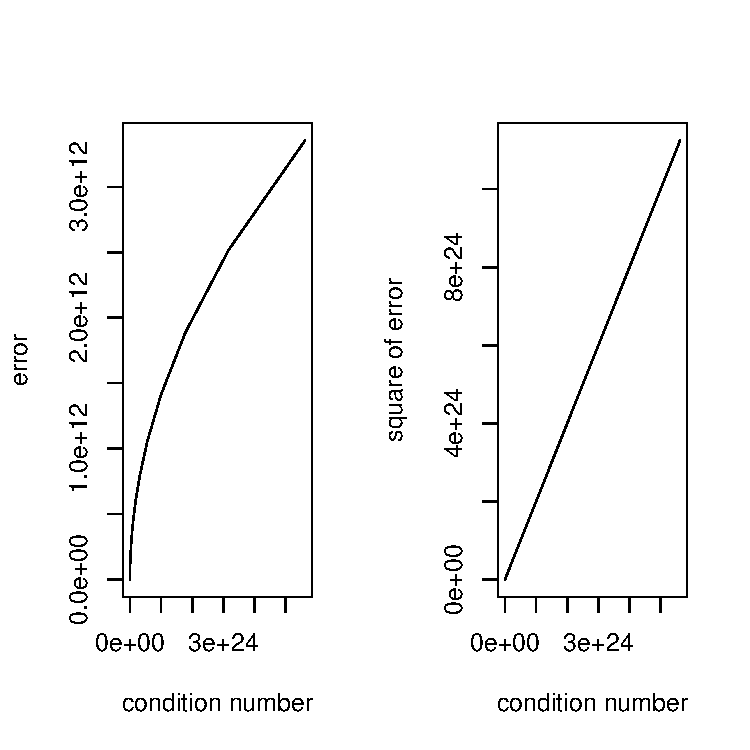
\includegraphics[width=\maxwidth]{figure/rchunk-6-1} 

\end{knitrout}
\end{document}
